\documentclass{article}
\usepackage[T1]{fontenc}
\usepackage{lmodern}
\usepackage[polish]{babel}
\usepackage{graphicx}
\usepackage{float}
\usepackage{placeins}
\usepackage{subcaption}

\usepackage[a4paper, margin=2.54cm]{geometry}

\title{Przetwarzanie Rozproszone - Projekt}
\author{Filip Gołaś 188776, Damian Jankowski 188597\\Patryk Korczak 188618, Tomasz Krezymon 189642}
\date{30 kwietnia 2023}

\begin{document}

\maketitle

\section{Wstęp}
Gra będąca tematem projektu będzie klonem popularnej gry przeglądarkowej agar.io stworzonej przez Matheusa Valadaresa i dostępnej pod adresem będącym jej nazwą.

\subsection{Zasady gry}
W grze bierze udział dowolnie duża ilość graczy umieszczona na planszy o ograniczonych rozmiarach. Na planszy
pojawiają się punkty, których zbieranie jest jednym z celów graczy reprezentowanych jako kolorowe okręgi o promieniu
odpowiadającym ilości zebranych przez gracza punktów. Gracze o rozmiarze znacznie większym od innych są w stanie
pochłaniać mniejszych od siebie graczy przejmując ich punkty i zmuszając do zaczęcia gry od nowa.

\section{Realizacja}
Gra będzie zaimplementowana z użyciem biblioteki graficznej SDL2. Komunikacja sieciowa będzie obsłużona z użyciem sieci klient-serwer.
Proces \textbf{serwera} będzie składał się z trzech głównych rodzajów wątków:
\begin{itemize}
    \item  \textbf{Wątek połączenia} - to on będzie nasłuchiwał próśb klientów o dołączenie do gry. Gdy prośba o dołączenie
    zostanie rozpatrzona klient otrzyma informacje potrzebne by połączyć się z wątkiem nasłuchiwania graczy, w
    tym port na który powinien wysyłać dalsze komunikaty i stałe w czasie jednej sesji parametry gry, oraz zostanie utworzony nowy wątek serwera nasłuchujący komunikatów od tego klienta.
    \item  \textbf{Wątek nasłuchiwania graczy} - w tym wątku serwer będzie nasłuchiwał komunikatów od graczy o prośbie o
    pojawienie gracza na planszy, detekcji kolizji oraz wykonywanych przez gracza ruchach oraz będzie aktualizował
    globalny stan gry na ich podstawie. Za obsługę każdego gracza będzie odpowiadał indywidualny personalny wątek nasłuchiwania gracza.    
    \item \textbf{Wątek odpowiedzi gry} - zadaniem tego wątku będzie rozsyłanie w sposób synchroniczny ze stałą częstotliwością informacji o zmianach stanu bytów występujących na planszy. Będzie się ona składała ze zmiennej długości listy wiadomości, które będą zawierać: zmianę kierunku ruchu, pojawienie się, zniknięcie, zmianę wyniku a co za tym idzie rozmiaru.
\end{itemize}


Do zadań każdego \textbf{klienta} będzie należało:

\begin{itemize}
    \item Wysyłanie prośby o połączenie do wątku połączenia serwera
    \item Odczytywanie wybranych przez gracza ustawień nazwy i koloru, które następnie będą wysyłane do serwera wraz z prośbą o pojawienie na planszy
    \item Odczytywanie ruchów gracza i informowanie o nich serwera
    \item Wykrywanie kolizji i informowanie o tym serwera
    \item Otrzymywanie od serwera informacji o globalnym stanie gry i aktualizowanie ich lokalnie
    \item Interpolacja ruchów innych graczy i tworzenie wszelkich innych interpretacji graficznych stanu gry
\end{itemize}

\section{Komunikacja}
Komunikacja zostanie rozwiązana w całości z użyciem protokołu TCP. Ponieważ wszelkie dane przesyłane między agentami są krytyczne i nie występują w nich żadne informacje chwilowe, aktualne jedynie przez krótki czas i zastępowane, więc każda utracona wiadomość skutkowałaby rozbieżnościami w stanach gry u agentów.
Rodzaje komunikatów używanych w komunikacji klient-serwer i serwer-klient:
\begin{itemize}
    \item \textbf{Prośba o połączenie} - gracz wysyła do serwera prośbę o dołączenie do gry oczekując przy tym odpowiedzi zawierającej port wątku nasłuchiwania graczy lub odmowy.
    \item \textbf{Odpowiedź na prośbę o połączenie} - serwer odpowiada podając informację o zaakceptowaniu lub nie, w pierwszym
    przypadku dołączony jest również numer portu na którym nasłuchiwane będą dalsze komunikaty od tego gracza.    
    \item  \textbf{Pojawienie się gracza} - gracz wysyła swoje imię i kolor okręgu, serwer decyduje czy gracz może pojawić się
    na planszy i po dodaniu klienta do listy graczy odpowiada przydzielonym graczu numerem ID. W dalszym ciągu gracz zaczyna normalnie otrzymywać zmiany stanu gry wraz z tickami serwera.
    \item \textbf{Wykonanie ruchu} - w momencie wciśnięcia/puszczenia przycisku klient wysyła komunikat o wciśniętych przyciskach, swoją aktualną pozycję, która będzie weryfikowana przez serwer oraz numer ostatniego odebranego Ticku będący wskazówką o momencie zajścia zdarzenia w przypadku skrajnych opóźnień połączenia.
     Poniżej zostały przedstawione graficznie dwie sytuacje, które mogą zajść w trakcie ruchów graczy:
     \begin{figure}[h]
        \centering
        \begin{subfigure}{.5\textwidth}
          \centering
          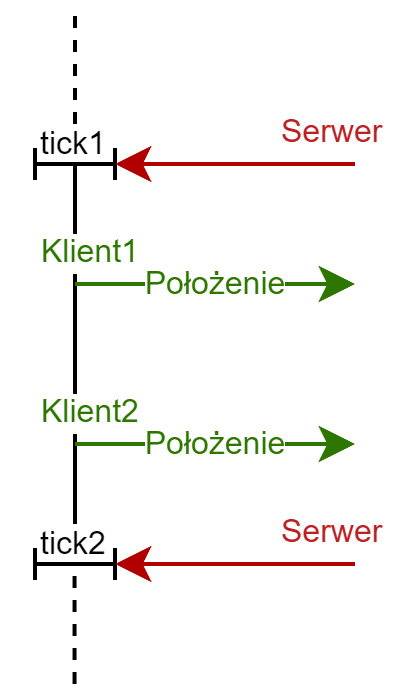
\includegraphics[scale=0.35]{ruch1.png}
          \caption{Ruch graczy z dobrym połączeniem}
          \label{fig:sub1}
        \end{subfigure}%
        \begin{subfigure}{.5\textwidth}
          \centering
          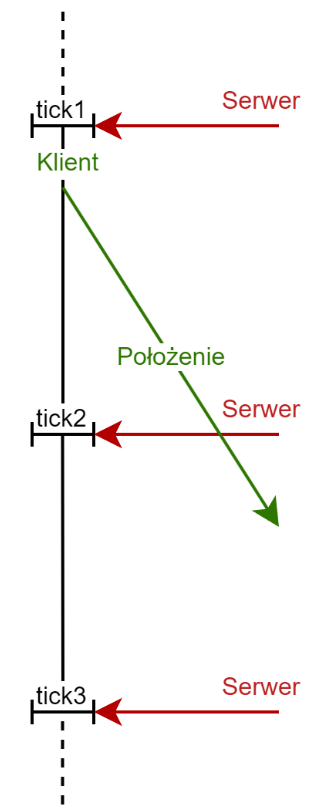
\includegraphics[scale=0.30]{ruch2.png}
          \caption{Ruch gracza ze słabym połączeniem}
          \label{fig:sub2}
        \end{subfigure}
        \caption{Diagramy przedstawiające ruch graczy podczas rozgrywki}
        \label{fig:test}
        \end{figure}

        Na diagramie (a) przedstawiono sytuację, w której klient 1 oraz klient 2 wykonują ruch. W takim przypadku
gracz 1 wysyła komunikat o swoim ruchu, a gracz 2 o swoim. Serwer otrzymuje oba komunikaty i aktualizuje
stan gry oraz rozsyła dalej do wszystkich graczy informacje o dokonanych przez ruchach w chwili następnego ticku serwera.

Diagram (b) przedstawia sytuację, w której gracz posiada słabe połączenie, dlatego jego wiadomość dociera
po odświeżeniu planszy przez serwer. Z tego powodu inni klienci wskutek niewłaściwej interpolacji ruchu tego gracza mogą doświadczyć nagłego przeniesienia się tego gracza w inne miejsce aby zachować synchronizację stanu gry z dokonanymi w rzeczywistości przez gracza ruchami.

    \item \textbf{Tick} - co tick serwer wysyła listę informacji o zmianach stanu bytów występujących na planszy opisaną wcześniej w wątku odpowiedzi gry serwera.

    \item \textbf{Kolizja} - w momencie gdy jeden z graczy wykryje kolizję z innym graczem lub punktem wysyła komunikat
    zawierajacy id swoje i gracza z którym zaszła kolizja oraz numer ostatniego otrzymanego od serwera ticku, będący wskazówką co do czasu zajścia zdarzenia. Serwer weryfikuje kolizję, porównuje rozmiary i decyduje
    o wyniku kolizji o czym klient dowiaduje się po otrzymaniu listy zmian w chwili następnego ticku, w której to znajdzie się informacja o wzroście jego wyniku, jego zniknięciu spowodowanym pochłonięciem przez wroga lub gdy serwer tak zadecyduje -- nie zawierającej żadnych zmian spowodowanych wykrytą przez niego kolizją. Stan gry oraz zawartość ekranu klienta nie będzie zmieniana w chwili wykrycia przez niego kolizji lecz dopiero po otrzymaniu odpowiedzi od serwera. 
    \begin{figure}[h]
        \centering
        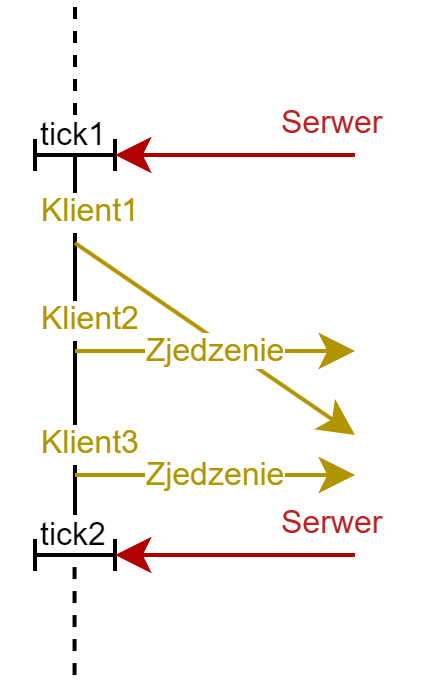
\includegraphics[scale=0.5]{jedzenie.png}
          \caption{Kolizja trzech graczy}
          \label{fig:sub3}
        \end{figure}
    \FloatBarrier
    Rysunek 2. przedstawia sytuację, gdzie trzech klientów wysyła informacje o zjadaniu innego gracza. Klient nr
1 i 2 wysyłają po sobie informację o zjedzeniu klienta nr 3 w ciągu jednego ticku. Z powodu słabego łącza
informacja od 1. gracza dociera później niż od 2. gracza. Z tego powodu serwer przyzna punkty graczowi,
którego informacja została odebrana wcześniej przez serwer, czyli 2. 

Co więcej, informacja o zjedzeniu innego
gracza przez gracza 3. zostanie zignorowana z racji, że dotarła do serwera najpóźniej, już po tym jak został
uznany za martwy przez serwer, więc jego wykrycie kolizji z innym graczem nie jest już według serwera prawdziwe. 

Dla gracza numer 1. oraz 3. sytuacja wyglądałaby identycznie gdyby ich opóźnienie było na tyle duże, że wiadomości dotarłyby później niż w tym samym ticku. Gdy do serwera dotrze przedawniona informacja o kolizji, której ten nie jest w stanie już zweryfikować również poskutkuje to jej zignorowaniem.
    \item \textbf{Prośba o rozłączenie} - wysyła ją klient, który chce opuścić grę. Serwer po jej otrzymaniu usuwa klienta z listy graczy zachowując jego gracza na planszy do pochłonięcia przez resztę uczestników
    \item \textbf{Komunikat błędu} - jest wysyłany przez serwer i zawiera wiadomość tekstową skierowaną do klienta informującą o zaistniałym problemie.
\end{itemize}
Problemy i sugerowane ich rozwiązania:
\begin{itemize}
    \item  \textbf{Brak odpowiedzi dla klienta ze strony serwera na prośbę o dołączenie}
    
    Po pewnym czasie oczekiwania stosowny komunikat i ewentualnie ponowna próba.
    \item  \textbf{Serwer nie otrzymuje prośby o pojawienie od połączonego klienta}
    
    Nie są podejmowane działania, taki gracz nie otrzymuje żadnych informacji dopóki nie poprosi o pojawienie,
    po określonym czasie taki klient jest rozłączany.
    \item \textbf{Serwer nie odpowiada na prośbę o pojawienie}
    

    Klient czeka określony czas, jeżeli w tym czasie nie zostanie otrzymany tick uznaje, że połączenie zostało
    zerwane, wymaga ponownego połączenia.
    \item  \textbf{Informacja o wciśniętych klawiszach nie dociera do serwera}
    
    
    Serwer nie reaguje, taki gracz dalej porusza się wedle ostatniej aktualizacji wciśniętych klawiszy będąc
    łatwym łupem dla aktywnych graczy. Gdy po pewnym czasie do serwera zaczną napływać znacznie opóźnione ruchy, pozycja gracza zostanie zaktualizowana, a reszta graczy otrzyma informacje o tych ruchach.
    \item  \textbf{Klient prosi o pojawienie mimo obecności na planszy}
    
    Tworzony i przypisywany jest klientowi nowy gracz, stary jest porzucany i zachowuje się tak jakby jego
    klient został rozłączony poruszając się w ostatnim otrzymanym kierunku.
    \item \textbf{Klient próbuje dołączyć mimo już obecności na liście graczy}
    
    Nie stanowi to problemu dla stanu gry. Serwer odsyła odpowiedni numer ID gracza. Klient pozostaje na liście graczy a serwer w dalszym ciągu oczekuje na prośbę o
    pojawienie się na planszy odnawiając jednak czas jaki serwer będzie czekał zanim rozłączy gracza.
    \item \textbf{Klient prosi o pojawienie nie będąc połączony}
    
    Serwer nie rozpoznaje tej wiadomości, jako że powinna ona być wysłana na indywidualny wątek klienta. Serwer nie odpowiada co zostanie odebrane przez klienta jako rozłączenie i będzie wymagać połączenia.
    \item \textbf{Klient wysyła ruch nie będąc połączony lub nie będąc na planszy}
    
    Serwer nie rozpoznaje tej wiadomości, jako że powinna ona być wysłana na indywidualny wątek klienta. Serwer nie odpowiada co zostanie odebrane przez klienta jako rozłączenie i będzie wymagać połączenia
    
    \item \textbf{Gracz wysyła ruch, będący poza obszarem, do którego gracz mógłby poruszyć się od ostatniego ticku serwera
    wynikającym z maksymalnej prędkości ruchu gracza i czasu między tickami}

    Ta sytuacja nie jest traktowana jako próba oszustwa. Wektor takiego ruchu jest skracany do maksymalnej
długości wynikającej z prędkości ruchu gracza i długości ticku. W takim wypadku dany gracz może po swojej stronie doznać teleportacji swojego obiektu gracza do poprawnej według serwera pozycji na planszy.

  \item \textbf{Czas przesyłania informacji o ruchu i pozycji od klienta do serwera przekracza znacznie okres ticku serwera}
  
  Serwer nie próbuje domyślać się jak powinny wyglądać ruchy tego gracza w przeszłości i zwyczajnie teleportuje go do odebranej pozycji, o ile jest poprawna. Klient, który wysyła tak opóźnione wiadomości jak i inni klienci mogą doświadczyć opóźnienia w ruchach i teleportacji obiektu gracza tego klienta.
\end{itemize}
\end{document}